\DiaryEntry{GCD - Algorithms (further stuff)}{2017-09-28}{Algebra}

The gcd algorithm is based on the following fact:

\bee
\gcd(a,b) = \gcd(a - b,b)
\eee

which we can repeat several times; i.e. $\gcd(a,b) = \gcd(a-b,b) = gcd(a-2b,b) = \cdots$ in order to arrive at

\bee
\gcd(a,b) = \gcd(a \bmod b, b)
\eee

This forms the basis for Euclid's Algorithm to calculate the gcd

\begin{verbatim}
gcd(a,b):
   if b=0: return a
   else return gcd(b, a mod b)
\end{verbatim}

We are interested in how many steps the algorithm needs (or at least the order of the number of steps) depending on the input. We make the following observation

\begin{theorem}
If $a \geq b$, then $a \bmod b < a/2$.
\end{theorem}

\paragraph{Proof.} We first note that $a \bmod b$ is in the interval from $0$ (when $a$ is a multiple of $b$) to $b-1$ (when $a$ is off a multiple of b by one). We can write $a = kb + (a \bmod b)$ with an integer $k$ chosen appropriately. In case of large $k$, the difference between $a$ and $b$ can be made arbitrary large (think of $64 \bmod 2$), the difference is smallest when $k=1$ ($k=0$ would violate the condition $a \geq b$). So we have $a=b + (a \bmod b)$ with $a$ and $b$ closest when the remainder is largest ($b-1$). So $a = b + b-1$ which we can rewrite as 

\bee
a=(a \bmod b)+1 + (a \bmod b) = 2 (a \bmod b) + 1 \rightarrow a \bmod b = \frac{a-1}{2}
\eee

and we arrive at $a \bmod b < \frac{a}{2}$ \qed

This shows that in every iteration of the gcd function (unless $b$ becomes zero), it is called with a second value being smaller than $a/2$. So in the worst case, the algorithm needs to perform $2 \log_2 a$ iterations. If $a$ is a number with $n$ digits, then $a = C 10^n$ with some constant $C$. We can rewrite this as $a = C' 2^n$ ($C'$ being another constant) and arrive at a number of division of $2 \log_2 (C' 2^n) = c n$, where we have also left off any constant terms. Therefore, the number of iterations / divisions of the Euclid Algorithm is linear in the number of digits.

The worst case complexity is reached in case $a$ and $b$ are two consecutive Fibonacci numbers. The following Figure shows the number of iterations / divisions  for a fixed value of $a=55$ (a Fibonacci number) versus $b$. It can be clearly seen that the maximum is reached for $b=34$, which is the preceding Fibonacci number. Another peak is at$b=21$ which is also a Fibonacci number. Towards the edges of the graph, the number of iterations / divisions falls off; in these cases the difference between $a$ and $b$ is so large that the algorithm stops after a few iterations. E.g. $\gcd(31,2) = \gcd(2,1) = \gcd(1,0) = 1$.


\begin{figure}[H]
	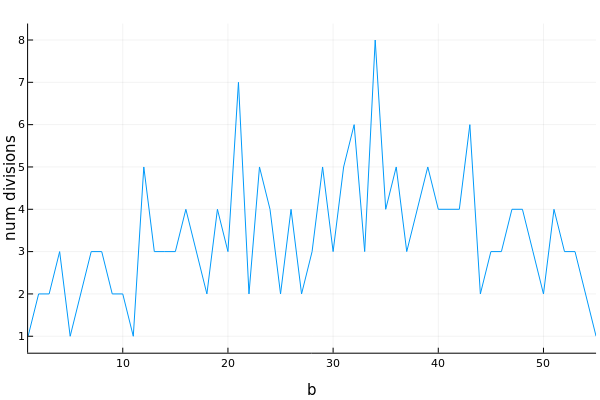
\includegraphics[scale=0.5]{images/gcd_num_div.png}
\end{figure}


\subsection{Worst Case Complexity}

We want to calculate the gcd of two subsequent Fibonacci numbers $F_{n+1}$ and $F_n$. We first make the following observation

\bee
F_{n+1} \bmod F_n = (F_n + F_{n-1}) \bmod F_n = F_n \bmod F_n + F_{n-1} \bmod F_n = F_{n-1}
\eee

because we can split the mod operation, $F_n \bmod F_n = 0$, and finally, $F_{n-1} < F_n$ and therefore $F_{n-1} \bmod F_n = F_{n-1}$.

Now let us calculate the gcd:

\bee
\gcd(F_{n+1}, F_n) = \gcd(F_n, F_{n+1} \bmod F_n) = \gcd(F_n, F_{n-1})
\eee

where we used the results from before. We can continue this game until we reach $\gcd(F_1, F_0) = \gcd(1,1) = 1$. This shows that two consecutive Fibonacci numbers are co-prime.